\documentclass{article}

\usepackage[margin=1in]{geometry}
\usepackage{graphicx} % Allow image/pdf includes
\usepackage{extramarks} % Extra header marks (continued on next page)
\usepackage{amsmath} % Math enhancements
\usepackage{amsthm} % Theorem typesetting
\usepackage{amssymb} % Extended symbol collection
\usepackage{tikz} % Graphical element creation
\usetikzlibrary{automata,positioning}
\usepackage{algpseudocode} % Algorithm layout
\usepackage{enumitem} % Enumerate (lists)
\usepackage{ragged2e} % Alternative alignment
\usepackage{gensymb} % Generic symbols (degree, etc)
\usepackage{empheq} % Allow \boxed around \begin{empheq}
\usepackage{color,soul} % Highlighting
\usepackage{booktabs} % Enhanced table creation
\usepackage{multirow} % Table multi row
\usepackage{mathtools} % Math enhancements
\usepackage{bm} % Bold math
\usepackage[mathscr]{euscript} % Script variables
\usepackage{cancel} % Cancel through text
\usepackage{color,soul} % Highlighting
\usepackage{mathtools}
\usepackage{multirow}
\usepackage{mathrsfs}
\usepackage{physics}
\usepackage{gensymb}
\usepackage{siunitx}
\usepackage{subcaption}
\usepackage[]{algorithm2e}
\usepackage{float}

\setlength\parindent{0pt} % No indents
\setlength{\parskip}{1em} % Paragraph skip

\newcommand{\vx}{\mathbf{x}} % x vector
\newcommand{\vy}{\mathbf{y}} % x vector

\newcommand{\pageTitle}{MEEN 644 - Homework 3}
\newcommand{\pageAuthor}{Logan Harbour}

\begin{document}

\title{\LARGE \textbf{\pageTitle} \vspace{-0.3cm}}
\author{\large \pageAuthor}
\date{\vspace{-0.6cm} \large \today \vspace{-0.4cm}}

\maketitle

\section*{Problem statement}

Complete

\section*{Preliminaries}

\subsection*{Two-dimensional heat conduction}

With two-dimensional heat conduction with constant material properties, insulation on the right and prescribed temperatures on all other sides, we have the PDE
\begin{equation}
	\begin{cases}
		k \pdv{^2T}{x^2} + k \pdv{^2T}{y^2} = 0\,,\\
		T(x, 0) = T_B\,,\\
		T(0, y) = T_L\,,\\
		T(0, L) = T_T\,,\\
		-k \pdv{T}{x} \Big|_{x = L} = 0\,,
	\end{cases}
\end{equation}
where
\begin{align*}
	T_B & \equiv 50~^\circ\text{C}\,, & T_L & \equiv 50~^\circ\text{C}\,, & T_T & \equiv 100~^\circ\text{C}\,.\\ 
	k & \equiv 386~\text{W/m}~^\circ\text{C}\,, & L & \equiv 0.5~\text{m}\,.\\
\end{align*}

We discretize the region on $x \times y = [0, L]^2$ by $N^2$ internal nodes with $\Delta x = x / N, \Delta y = y / N$.

\subsection*{Equation discretization}

\subsubsection*{Internal control volume equations}

Integrate over an internal control volume $(i,j)$ and use the two node formulation for the derivative to obtain
\[
	k \Delta y \left[\frac{T_{E_{ij}} - T_{P_{ij}}}{\Delta x} - \frac{T_{P_{ij}} - T_{W_{ij}}}{\Delta x}\right] + k \Delta x \left[ \frac{T_{N_{ij}} - T_{P_{ij}}}{\Delta y} -\frac{T_{P_{ij}} - T_{S_{ij}}}{\Delta y} \right] = 0\,, \quad (i, j) \in [2, 3, \ldots, N]^2\,.
\]
Collect like terms and modify the index to obtain
\begin{equation}
	\label{eq:internal}
	T_{i,j} a_p - T_{i, j+1} a_n - T_{i+1, j} a_e - T_{i, j-1} a_s - T_{i-1, j} a_w = 0\,,\quad (i, j) \in [2, 3, \ldots, N]^2\,,
\end{equation}
where
\[
	a_n \equiv \frac{k \Delta y}{\Delta x}\,, \quad a_e \equiv \frac{k \Delta x}{\Delta y}\,, \quad a_s \equiv \frac{k\Delta y}{\Delta x}\,, \quad a_w \equiv \frac{k\Delta x}{\Delta y}\,, \quad a_p \equiv a_n + a_e + a_s + a_w\,.
\]

The remaining equations are solved similarly.

\subsubsection*{Bottom internal control volume equations}

\begin{equation}
	T_{i,2} (a_n + a_e + 2a_s + a_w) - T_{i,3} a_n - T_{i+1,2} a_e - T_{i-1, 2} a_w = 2 T_B a_s\,, \quad i \in 3, 4, \ldots, N\,.
\end{equation}

\subsubsection*{Bottom left control volume equation}
\begin{equation}
	\label{eq:bot_left}
	T_{2,2} (a_n + a_e + 2 a_s + 2 a_w) - T_{2,3} a_n - T_{3,2} a_e = 2 T_B a_s + 2 T_L a_w\,.
\end{equation}

\subsubsection*{Left internal control volume equations}

\begin{equation}
	T_{2,j} (a_n + a_e + a_s + 2a_w) - T_{2,j+1} a_n - T_{3,j}a_e - T_{2,j-1} a_s = 2 T_L a_w\,, \quad j \in 3, 4, \ldots, N\,.
\end{equation}

\subsubsection*{Top left control volume equation}

\begin{equation}
	T_{2, N+1} (2a_n + a_e + a_s + 2a_w) - T_{2,N} a_s - T_{3,N+1} a_e = 2 T_T a_n + 2 T_L a_w\,.
\end{equation}

\subsubsection*{Top internal control volume equation}

\begin{equation}
	T_{i,N+1} (2a_n + a_e + a_s + a_w) - T_{i+1,N+1}a_e - T_{i, N} a_s - T_{i-1,N+1} a_w = 2 T_T a_n\,, \quad i \in 3, 4, \ldots, N\,.
\end{equation}

\subsubsection*{Top right control volume equation}

\begin{equation}
	T_{N+1, N+1} (2a_n + a_s + a_w) - T_{N+1, N} a_s - T_{N, N+1} a_w = 2 T_T a_n\,.
\end{equation}

\subsubsection*{Right internal control volume equations}

\begin{equation}
	T_{N+1, j} (a_n + a_s + a_w) - T_{N+1, j+1} a_n - T_{N+1, j - 1} a_s - T_{N, j} a_w = 0\,, \quad j \in 3, 4, \ldots, N\,.
\end{equation}

\subsubsection*{Bottom right control volume equation}

\begin{equation}
	T_{N+1, 2} (a_n + 2 a_s + a_w) - T_{N+1, 3} a_n - T_{N, 2} a_w = 2 T_B a_s\,.
\end{equation}

\section*{Results}

\subsection*{Part a}

\begin{figure}[H]
	\centering
	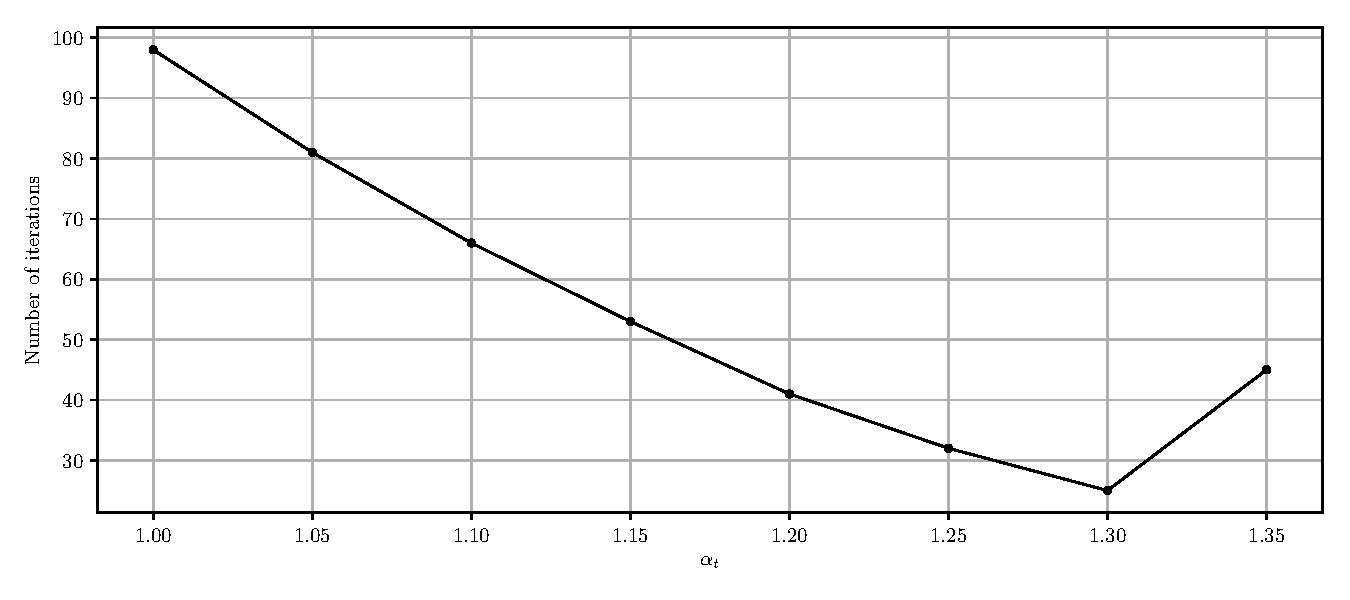
\includegraphics[width=\linewidth]{../python/iterations}
	\caption{Plot of the required iterations for each over relaxation factor.}
	\label{fig:iterations}
\end{figure}

\subsection*{Part b}

\begin{figure}[H]
	\centering
	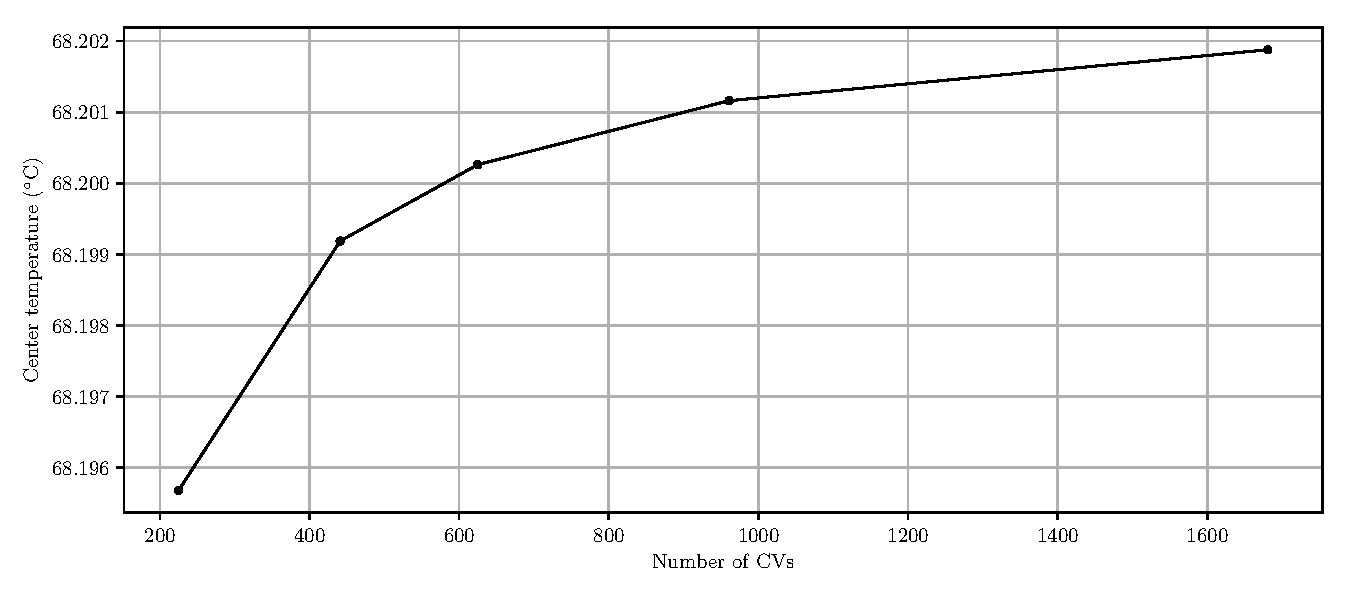
\includegraphics[width=\linewidth]{../python/center}
	\caption{Plot of the center temperature with mesh refinement.}
	\label{fig:center}
\end{figure}

\subsection*{Part c}

\begin{figure}[H]
	\centering
	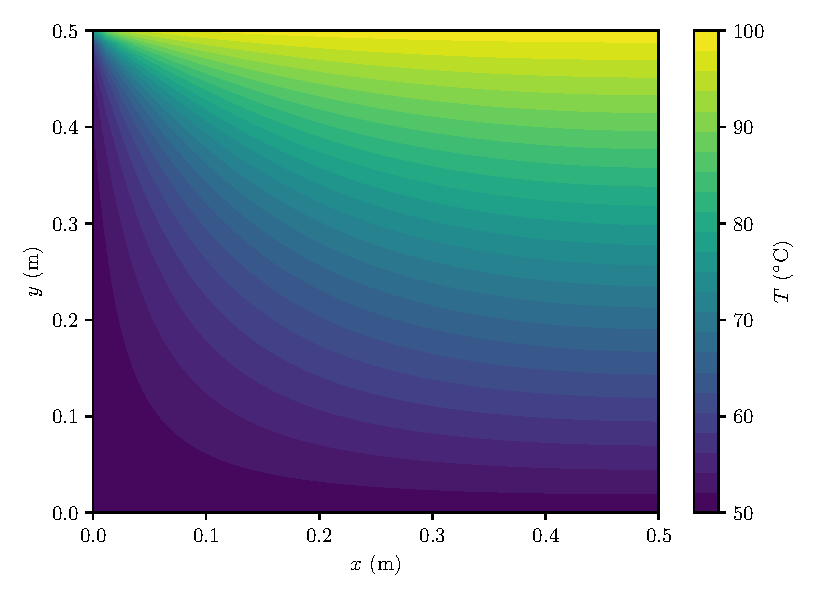
\includegraphics[width=0.7\linewidth]{../python/solution}
	\caption{Plot of the solution with $41 \times 41$ CVs.}
	\label{fig:solution}
\end{figure}

\end{document}
